\documentclass[12pt]{article}

\usepackage{sbc-template}

\usepackage{graphicx,url}
\usepackage{hyperref}
\usepackage{nicematrix}

\usepackage{array}

%\usepackage[brazil]{babel}   
\usepackage[utf8]{inputenc}  

\usepackage{seqsplit}

     
\sloppy

\title{Mitigating Code Duplication in the Linux Kernel}

%% Double-Blind review
%%%%%%%%%%%%%%%%%%%%%%
%\author{Luan Arcanjo\inst{1}, Marcelo Spessoto\inst{1}, David Tadokoro\inst{1}, Paulo Meirelles\inst{1}}

%\address{FLOSS Competence Center\\
%        Institute of Mathematics and Statistics\\
%        University of São Paulo
%  \email{\{luanicaro,marcelomspessoto\}@usp.br,paulormm@ime.usp.br}
%}

\begin{document} 

\maketitle

\begin{abstract}
The vast scale and continuous evolution of the Linux kernel make its maintenance a complex undertaking, where code duplication remains a persistent challenge that can hinder development and introduce bugs. This paper presents a multimethod ethnographic study investigating the socio-technical dynamics of contributing to the Linux kernel by mitigating identified redundancies. To support this investigation, we developed \texttt{anonymous-tool}, a command-line utility for detecting function-level duplications, offering a concrete entry point for new contributors. Our ethnographic approach, including participant and non-participant observations, demonstrated that addressing duplications is viable for lowering the contribution barrier. This point is evidenced by the main author and 7 of 11 (64\%) student groups having their patches accepted into the kernel, collectively removing 991 lines of duplicated code. Moreover, the study also reveals a more complex reality beyond simple clone removal: an analysis of maintainer feedback on both accepted and rejected patches highlights a nuanced understanding of code quality within the Linux kernel community, where the benefits of eliminating duplication are carefully weighed against factors such as readability, the introduction of new abstractions, and the specific context of the code.
\end{abstract}


\section{Introduction}
\label{sec:introduction}

Coordinating hundreds or thousands of developers working on a software product is complex. Creating similar or even completely duplicated code is a frequent and often unavoidable outcome. Excessive duplication can negatively impact the maintainability of a project. When duplications occur, any change to a repeated code segment typically requires manual replication across all other copies. Developers must, therefore, remain constantly vigilant to synchronize different parts of the codebase, which is a highly error-prone and seemingly simple responsibility. With many duplications, modifications become slow, complex, and fragile. Removing or refactoring duplicated code demands great care to preserve the original behavior. Even minor mistakes can introduce subtle state changes that may lead to serious problems in the future.

The Linux kernel is a foundational Free/Libre and Open Source Software (FLOSS) project, a vital component of the world's digital infrastructure. Its maintenance is a massive undertaking, encompassing over 28 million lines of code and involving contributions from over twenty thousand developers. Within this context, code duplication remains a significant challenge,  reducing the code readability and increasing the risk of introducing bugs~\cite{harmone,harmtwo}. This issue is particularly prominent in kernel device drivers, which account for over 66\% of the Linux kernel source code.

The detection of code duplication, or \textit{code clones}, has been a research topic for decades~\cite{firstman}. The literature offers a widely accepted taxonomy that classifies clones into four types based on their similarity, from exact copies (Type-1) to semantically equivalent but syntactically different fragments (Type-4)~\cite{litreview}. Several detection techniques have emerged, including textual, token-based, tree-based, and graph-based approaches~\cite{litreview}. These efforts have culminated in state-of-the-art techniques, such as the graph-based approach proposed by Liu et al.~\cite{tailor}.

To address the code duplication issue, we developed \texttt{anonymous-tool}, a command-line tool designed to support Linux kernel maintenance by detecting and analyzing function-level duplications. This paper presents a multimethod ethnographic study to validate the tool capabilities in identifying duplications and supporting contributions to the Linux kernel by mitigating redundant code. Therefore, the study investigates how the Linux kernel community perceives the code quality related to code clones. Our findings indicate that maintainers consider not only duplication but also factors such as readability and appropriate levels of abstraction regarding code maintainability.

Ethnography is a well-established qualitative research method used to understand people, their cultures, and their work practices~\cite{bookethno}. It enables researchers to gain insights into values, beliefs, and practices from the perspective of community members~\cite{ethnosoft}.  
In this study, we first adopted a participant observation approach, where the main author actively engaged in mitigating code duplications while documenting the process and outcomes. Later, we followed a non-participant observation involving students tasked with resolving duplications identified by the tool. These combined studies showed that \texttt{anonymous-tool} can collaborate to reduce the entry barrier for new contributors. The student groups and the main author used the tool to guide their initial contributions to the Linux kernel.


\section{The Linux Kernel}

The Linux kernel is a monolithic system organized into subsystems, such as the process scheduler, memory management, and device drivers. Each subsystem typically has a dedicated maintainer or a team of maintainers overseeing its development and managing contributions. The development process is coordinated through the Git version control system. Contributions are formatted as patches, text documents that outline the differences between two source code versions. These patches are then submitted to the relevant Linux mailing lists for public review and discussion.

This study focuses on two of these subsystems, selected to represent different contexts for contribution. We explore the AMD Display driver, chosen for its importance within the hardware ecosystem, which is responsible for enabling AMD GPU functionality in Linux. This subsystem is substantial, with over 391,000 lines of code across more than 1,089 files. We also investigate the Industrial I/O (IIO) subsystem, often considered an accessible entry point for new contributors. The IIO subsystem provides support for devices that perform analog-to-digital or digital-to-analog conversions\footnote{\href{https://kernel.org/doc/html/v4.14/driver-api/iio/intro.html}{kernel.org/doc/html/v4.14/driver-api/iio/intro.html}} and contains over 281,772 lines of code in more than 755 files.

\section{Anonymous-tool}

We developed \texttt{anonymous-tool}, a command-line tool designed to detect and analyze function-level code duplication within the Linux kernel to support our investigation. Released under the MIT license, \texttt{anonymous-tool} employs a two-stage architecture that separates the computationally intensive task of finding duplicates from the process of querying the results. The first stage, the Preprocessor, analyzes the entire codebase, parses C functions, and stores identified duplicates in a database. The second stage, the Query Responder, uses this database to retrieve information about the identified duplications quickly.
%The tool is available at \textit{\href{https://github.com/arkanjo-tool/arkanjo}{github.com/arkanjo-tool/arkanjo}}.

\texttt{Anonymous-tool} is designed for the specific challenges of the kernel, with a focus on scalability to handle its size and prioritizing duplications that impact maintainability. The tool's primary role in this study was to provide a concrete entry point for new contributors by identifying function-level duplications to address. Figure~\ref{fig:diagrama} illustrates the tool's architecture. The tool uses a text similarity method that applies TF-IDF vector embedding, implemented with the Gensim library~\cite{gensim}, and computes cosine similarity to detect clones.

\begin{figure}[ht]
\centering
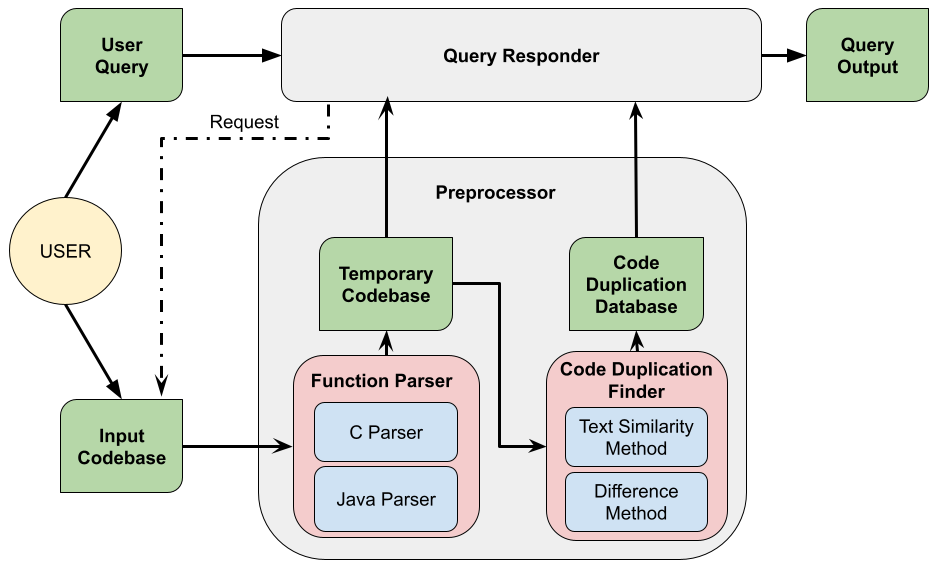
\includegraphics[scale=0.33]{diagrama_mestrado}
\caption{Architecture diagram with the tool components
}
\label{fig:diagrama}
\end{figure}

\section{Participant Observation Study}
\label{sec:participant}

To investigate whether we can use the \texttt{anonymous-tool} tool to find ways to contribute to the Linux kernel, we conducted a participant observation experiment in the second semester of 2024, where we acted as first-time contributors to the AMD Display driver, collecting artifacts of our experience in the process.

In the AMD Display driver codebase, we executed the \texttt{anonymous-tool}. We manually analyzed the biggest duplications regarding the number of lines and found two duplicated function pairs that we judged interesting to try to mitigate. We have chosen to approach the biggest duplications as proof of concept so that we can make significant impacts. 

The first duplicated function pair chosen is function \textit{offset\_to\_id} on files \textit{dc/gpio/dcn32/hw\_translate\_dcn32.c} and \textit{dc/gpio/dcn315/hw\_translate\_dcn315.c}. The second duplicated function pair is function \textit{phy\_id\_to\_atom} in file 
\textit{ \seqsplit{dc/bios/dce110/command\_table\_helper\_dce110.c}} and \textit{\seqsplit{dc/bios/dce60/command\_table\_helper\_dce60.c}}.
Hereafter, the mitigation on \textit{offset\_to\_id} will be referred to as mitigation 1, and the mitigation on 
\textit{phy\_id\_to\_atom} will be referred to as mitigation 2.



Given the two duplicated function pairs, we observed that the files in the functions 
contain multiple other duplications. Thus, we proposed a simple systematic approach 
to mitigate all the functions duplicated in the context, not just the duplicated 
function pairs. 
After we approached the duplications with the systematic strategy, for the duplicated 
function pairs that had successfully mitigated the duplication, we sent patches to the 
AMD Display driver email list to validate the mitigations and see the maintainer's opinion 
while documenting the process and our impressions.
The systematic approach is defined below. 

In C programming, communication between source files is achieved by creating header files that specify 
libraries~\cite{Cbook}. Since the Linux kernel is primarily written in C, we eliminated code duplications 
by consolidating duplicated code into a single library, which would replace instances of 
duplication across the codebase.

For each duplicated function pair, for each function in the pair, we used the \texttt{anonymous-tool} to locate all duplications of the function in the codebase, as it may have been duplicated more times than the two occurrences contained in the duplicated function pair. 
This strategy resulted in a collection of duplicated functions and corresponding code files.

To identify shared code more effectively, we extended this approach to search for other common 
functions across all collection files. We then applied specific refactoring methods to each shared 
function. If the functions were identical across files, we removed the duplicates and created a single 
function in the library. If modifications existed, we applied case-specific refactoring.

\subsection{Results}
\label{subsec:participantresults}


Table \ref{tab:patch} summarizes the impact of the mitigations in terms of 
files and lines changed and the refactoring method used. The following sections present our experience and learning for each mitigation.

\begin{table}
\centering
\caption{Refactor methods used and mitigation metrics in the participant-observation experiment.}
\begin{tabular}{ | m{20mm} | m{15mm} | m{15mm} | m{15mm} | m{40mm} | }

\hline

\textbf{Mitigation} & \textbf{Files changed} & \textbf{Lines added} & \textbf{Lines removed} & \textbf{Refactoring methods used}
\\ \hline 

1 & 13 & +224 & -753 & Parameterize Method, Extract Method  \\ \hline
2 & 8 & +114 & -520 & None \\ \hline

\hline
\end{tabular}

\label{tab:patch}
\end{table}

\subsubsection{Mitigation 1}

In the systematic approach, we found that the \textit{offset\_to\_id} function 
exists in 10 code files, enclosing multiple GPU architectures. The duplicated 
functions are not exactly equal, as some minimal specific logic is applied to each GPU architecture. To address this issue, we used the extract method to 
break the function into smaller parts and the parameterized method to address 
the specific logic for the GPUs.

We reached a point where we had a scratch on how to mitigate the duplications found, but we could not complete the refactoring to a state capable of submitting as a patch to the driver. We found that the configuration files on the AMD Display driver are designed to be imported at compilation time using \textit{\#define} macros. The configuration files' design choice makes refactoring duplications on generic approaches trickier, as refactoring code that depends on these files requires significant refactoring of the configuration files' design and deep knowledge of the codebase, which we, as first-time contributors, do not have. Thus, we opted not to continue investigating this mitigation.

\subsubsection{Mitigation 2}

Using the systematic approach, we found that the \textit{phy\_id\_to\_atom} function exists in five code files, and two other functions are duplicated 
in those five code files. All functions across the files were exactly equal, 
so there was no need to apply the refactoring methods presented in the literature. 
The refactoring was resumed to create a generic library and fix the compilation targets.

The code files in the second mitigation do not depend on configuration files. Thus, 
we did not face the same issues during the first mitigation. Refactoring the code 
to mitigate duplications reached a point we judged was good enough to submit as a 
patch to contribute to the AMD Display driver code quality. Thus, we moved to send 
the refactoring to the driver maintainers as a patch, documenting our findings and experiences 
on the process.

\begin{figure}
\centering
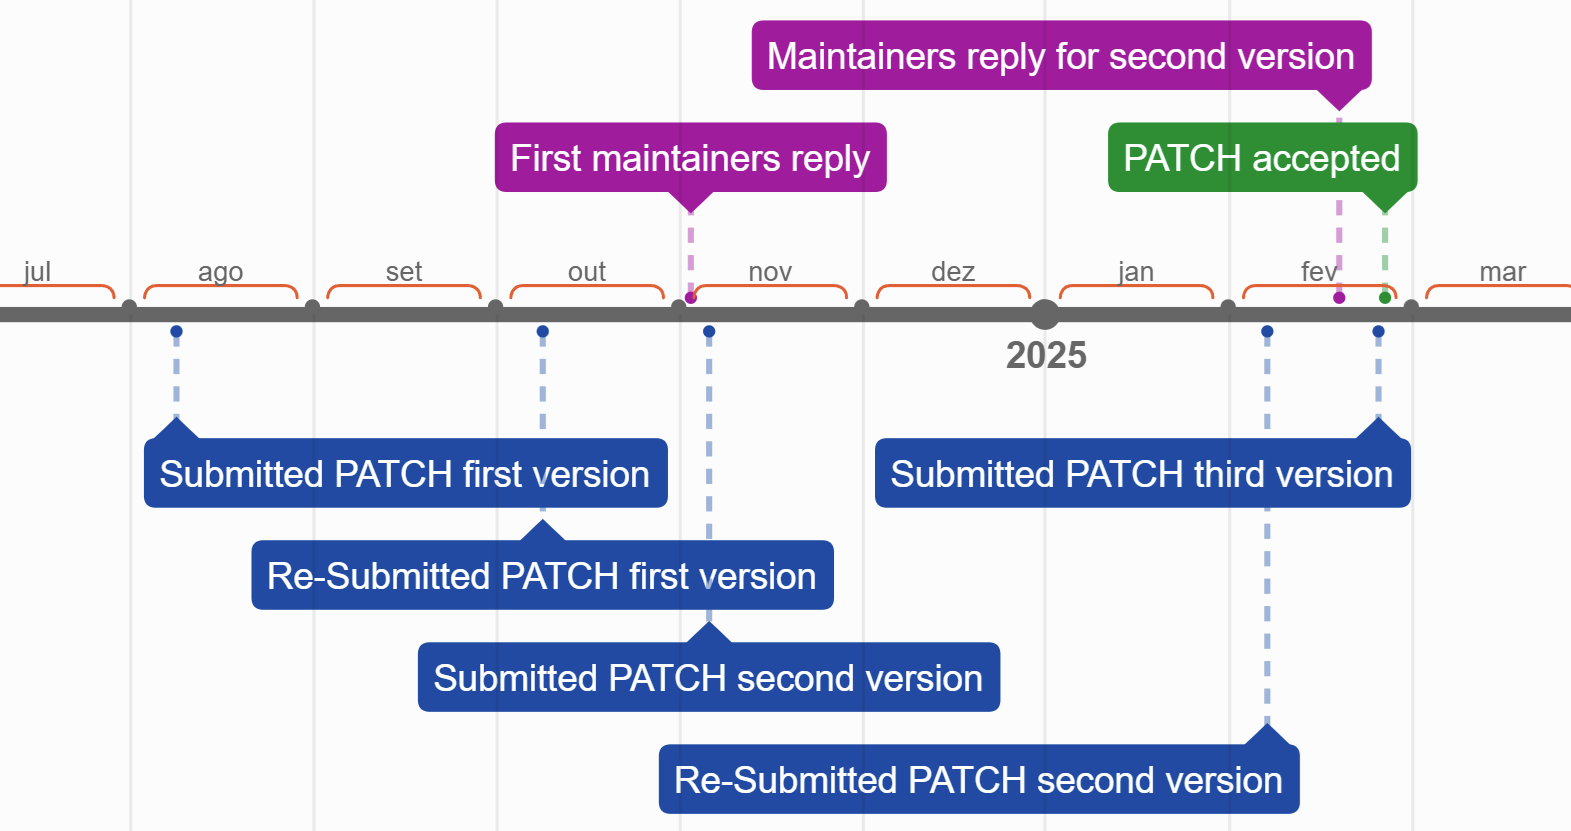
\includegraphics[scale=0.45]{timeline_patch}
\caption{Timeline of the PATCH submission process}
\label{fig:timeline}
\end{figure}

The experience of submitting a patch was not as we expected. The process took 7 months and 16 days, significantly slower than expected. We initially submitted the patch on August 9, 2024, but we did not receive replies. Thus, we had to resend it on October 9, 2024. We received an initial response on November 3, 2024, requesting minimal changes. We submitted a second version with the requested changes on November 16, 2024. We did not receive replies initially and will need to resend the patch on February 7, 2025. We received a reply on February 11, 2025, asking for additional changes. We sent a third version on February 24, 2025, and the patch was accepted and integrated into the kernel codebase on February 25, 2025. Figure \ref{fig:timeline} illustrates the timeline of the patch submission.

After the initial reply from the maintainers, we observed that the review process became more responsive. We hypothesize that once a patch receives initial attention, it is more closely tracked by maintainers. Another contributing factor to the initial delay could be the maintainers' workload at the time of the first submission.

We discussed the Display driver with our point of contact at AMD to understand the reason for the slow patch submission process. We learned that some of the code in the driver is shared across all operating systems that support the implemented GPUs. This fact creates a complex process within AMD to format and submit changes across the supported systems while simultaneously implementing measures to mitigate errors. Additionally, we comprehended that AMD Display driver developers can not view duplicated code negatively, as we understand it is a good practice in software engineering. One example shared with us is that duplicated code enhances the independence of GPU driver code, allowing developers to make changes to a specific GPU without needing to test compatibility with others. This approach helps save a significant amount of time and effort.

Regarding the patch changes requested for the second version, the maintainers only asked for minor changes to align with code style, correct license use, and best practices that were initially unknown. For the change requested on the third version, the maintainers asked us to move the functions created in the generic library to an existing file instead of creating a new one.
%\footnote{Patch submitted: \href{https://lore.kernel.org/all/20250225015532.303032-1-luanicaro@usp.br/}{lore.kernel.org/all/20250225015532.303032-1-luanicaro@usp.br}}.

\section{Non-participant Observation Study}

A core dynamic of the course (concurrently for undergraduate and postgraduate studies) is to have students make a practical contribution to a free software project. In the first semester of 2025, the professor teaching the course, who is also the advisor of this work, identified an opportunity to leverage the \texttt{anonymous-tool} tool within this existing pedagogical structure. As a contribution option, the professor proposed that students mitigate code duplications found in the Linux kernel. The professor drove this initiative as a practical course activity, and the author of this thesis was not involved in using the tool to identify duplications or in developing approaches to mitigate them. The tasks were carried out entirely by the course staff and the students.

The course had 37 students (25 undergraduate and 12 graduate), who were asked to form groups of 
two or three members. To assist students in this task, the professor and teaching assistants prepare multiple 
alternatives for contributing to free software projects, including simpler contributions such as 
updating documentation or fixing code style issues. In this context, two new options related to the 
\texttt{anonymous-tool} were proposed alongside the others.

For the first anonymous-tool-related alternative, a teaching assistant ran the tool on the IIO subsystem twice, creating two lists of duplicated function pairs, one with a 100\% similarity threshold and the other with a 90\% similarity threshold. Then, the following process happened to both lists:

\begin{enumerate}
    \item The teaching assistant filtered the lists to keep only duplicated pairs that happened in the same file, because the IIO subsystem is very decentralized, and a duplication between two different devices may involve the cooperation of different maintainers and/or the unification of totally different interfaces;
    \item The teacher assistant removed duplications that were too short and would not represent a significant change for a patch application;
    \item The teacher assistant manually ranked code duplications and marked some duplications with insights based on personal opinion and perceptions over the remaining entries. This was done to guide students so that they could approach the technical debt with a greater chance of having their contribution merged into the code.
\end{enumerate}

The students' task was to select a recommended entry from the list, refactor the code to eliminate these specific duplications, and then submit their patches to the IIO maintainers for review.

For the second alternative, students were offered an experience similar to our initial participant 
observation. In this model, the students were responsible for the entire workflow: executing the 
\texttt{anonymous-tool} on the AMD display driver, independently analyzing the results to identify a duplication 
to fix, creating a patch to mitigate it, and sending the patch to the driver's maintainers.

Of the students who chose to work on the \texttt{anonymous-tool}-related tasks, 23 (16 undergraduate and 7 graduate) 
formed 11 groups to pursue the first alternative. One graduate student also opted for the second alternative. Notably, none of these students had prior experience contributing to the Linux kernel, making this their first attempt to submit a patch as newcomers to the project.
%TODO: ver na versão final incluir o patch do Lucas (Octavio e Fernando)

The groups were requested to document their experiences and approaches to refactoring the duplications, as well as their experiences submitting a patch to the Linux kernel, in blogs. We analyzed these blogs to understand the refactoring patterns used to mitigate duplications, the experience of sending patches, and the opinions of subsystem maintainers on the mitigations.

\subsection{Overview of the submitted patches}

Table \ref{tab:stu} summarizes the student groups' mitigation approaches. It contains the information about the chosen subsystem and the similarity threshold for groups that opted for the first approach. Each entry also has the patch status, refactoring method, and code diff corresponding to the final patch versions before it was dropped or accepted into the code base. The code diff for a patchset corresponds to the sum of added and removed lines of each of its patches.

\begin{table}[ht]
\centering
\caption{Refactor methods used and metrics of the students' mitigations.}
\resizebox{1\linewidth}{!}{%
\begin{NiceTabular}{ | c | m{20mm} | m{25mm} | m{30mm} | m{46mm} | m{28mm} | }[hvlines]
\hline
\textbf{Group} & \textbf{Subsystem} & \textbf{Similarity} & \textbf{Patch Status} & \textbf{Refactoring Method} & \textbf{Code Diff} \\
\hline

1 & IIO & 100\% & Dropped (v2) & Undefined & +7/-14 \\ \hline
2 & IIO & 100\% & Dropped (v1) & Parameterize method & +23/-27 \\ \hline
3 & IIO & 100\% & Accepted (v1) & Parameterize method & +12/-30 \\ \hline
4 & IIO & 100\% & Accepted (v3) & Undefined & +2/-7 \\ \hline
5 & IIO & 90\% & Accepted (v1) & Parameterize method & +17/-70 \\ \hline
6 & IIO & 90\% & Dropped (v1) & Parameterize method & +95/-92 \\ \hline
7 & IIO & 90\% & Accepted (v3) & Extract method & +20/-36 \\ \hline
8 & IIO & 90\% & Accepted (v4) & Extract method & +20/-16 \\ \hline
9 & IIO & 90\% & Accepted (v6) -- Partially & Parameterize method & +149/-243 \\ \hline
10 & IIO & 90\% & Dropped (v1) & Undefined & +32/-58 \\ \hline
\Block{2-1}{11} & IIO & 100\% & Dropped (v1) & Inline method & +2/-12 \\ 
& AMD & 90\% & Accepted (v2) & Undefined & +90/-489 \\ \hline

\end{NiceTabular}%
}
\label{tab:stu}
\end{table}

Seven groups applied the parameterized refactor method, two groups used the extractor method, and one group applied the inline method to their approaches to mitigate their duplications. Four patches do not contain a refactoring technique defined in the literature (undefined). Six groups had their patches accepted and fully merged into Linux; four groups had their patches dropped; one group has its patchset partially applied and is still working on patch submission, currently in the sixth version of the patch when this document was written, but we can also consider this case as accepted.

Groups 1 and 4 have worked in similar duplications, where two functions are involved: one to determine if a register is volatile and the other to determine if it is writable. These are two functions that return opposite Boolean results. Group 1 initially addressed the problem using the extract method, while Group 2 used macros. After feedback from maintainers, both solutions converged to keep one of the functions while changing the content of the other to return a negated query of the former function. However, by the end of the feedback cycle, maintainers considered the patch from Group 1 irrelevant, while the patch from Group 4 was accepted. The reason is that Group 1 has chosen to apply the refactoring to a device that contains a register that is both read-only and non-volatile. Thus, the technical debt selected by Group 1 was not merely a duplication but an incorrect implementation of the method.

Groups 3, 6, and 10 created a struct to encapsulate the parameters and mitigate duplication when applying the parameterized method. The patches from Groups 6 and 10 were rejected by the same maintainer who approved the patch from Group 3. The maintainer's justification for rejecting the patch from Group 6 is that it proposes to fix duplication while adding more lines than removing, and is not convincing enough in other aspects, such as readability. The reason for rejecting the patch from Group 10 is that they refactored code files with simple context; therefore, adding a layer of abstraction to remove duplication decreases code readability without clear gains in codebase quality. The maintainers' feedback for Group 10 was:
\begin{quote}

\textit{``A few comments inline, but overall I'm not sure the code reduction is sufficient to cover the resulting loss of readability. Sometimes a switch is simply clearer than a partial look-up table.''}

\textit{``So nice idea, but I'm not seeing it as being a good move for this particular code. I'd be slightly interested to see the optimized output of the two approaches, but this is far from a high-performance path, so we care a lot more about readability here.''} 
\end{quote}


Interestingly, both groups addressed duplications across initialization functions for different devices, where code readability is vulnerable to refactoring methods. In contrast, Group 3 tackled the duplication of a simple iterative algorithm, which also contained a bug that could be inferred by inspecting both functions. In this case, the group refactored code from a more critical technical debt and took the opportunity to fix an unnoticed incorrect behavior.


%\begin{figure}
%\centering
%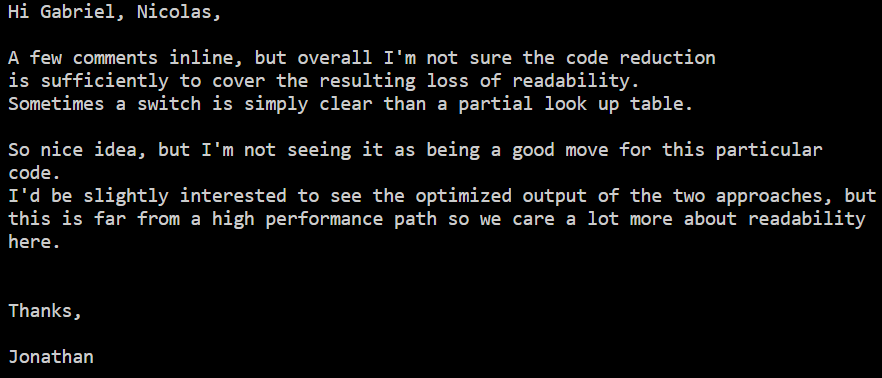
\includegraphics[scale=0.8]{group_10_reply}
%\caption[Maintainers' Feedback on Group 10 Patch]{
% Maintainers' Feedback on Group Ten's Patch
%}
%\label{fig:group_10_reply}
%\end{figure}

Groups 7 and 8 used the extract method to approach the mitigations. Group 8 sent the mitigations to the maintainers, and the code changes were approved, with minor requested changes in code style and smaller errors fixed. For Group 7 mitigation, the maintainer initially rejected the proposed patch but suggested a new refactoring approach: applying the extraction method refactoring to the duplicated code to an existing helper function. After the feedback cycle, maintainers accepted the patch in version 3.

Group 9 initially approached the selected duplication with a parameterized method, but after entering the feedback cycle, it was revealed that the problem represented a much more complex technical debt. The patch is still under development, currently at version 6, and has been separated into a 4-patch patch set, where half of them have been applied, and the remaining entries are receiving suggestions. Fortunately, maintainers are receptive and provide constant feedback; the contribution is expected to be fully merged if the students do not abandon the current work.

Group 11 is the student who executed the tool and completed the process of identifying duplications. The student identified a duplication in the driver that occurred across eighteen code files, creating a patch to remove approximately four hundred lines of duplicated code. The student sent the mitigations to the maintainers, and their feedback pointed to fixing the warning in the code without arguing about removing the duplications. After addressing the issue, the patch was applied. This student also contributed to IIO, tackling a code duplication with inline method refactoring. This one, however, was received with more skepticism by the maintainer, and the student dropped the contribution because he did not think the feedback instructions were clear enough.

Analyzing the students' approaches to the duplications and the maintainers' feedback, we saw that people without previous experience in Linux kernel development could approach duplications found by the \texttt{anonymous-tool} and become contributors to the kernel. We observed that not all duplications 
are viewed as code of bad quality, with maintainers analyzing the trade-off between the purpose of the duplicated code, code readability, and the levels of abstraction added to address the duplications.

\subsection{Statistics of the contributions}

The eleven groups, which have submitted 11 contributions to the IIO subsystem, have collectively requested the insertion of 379 lines and the deletion of 605 lines in the subsystem, representing an average of 34.45 lines added and 55 lines removed per contribution.

Considering the sum of fully merged contributions, we have a code diff value of +51/-143, with an average of +12.75/-35.75. This ratio is better than dropped contributions, which have a total of +179/-219 with an average of +29.83/-36.5.

It is also possible to notice a difference based on the similarity threshold used to detect duplications. The proposed patches to address 100\%-similarity duplications summed up to +46/-90 (average of +9.2/-18). For a 90\% value, the result was a total of +333/-515 with an average of +55.5/-85.83. The 90\% value enabled \texttt{anonymous-tool} to identify less strict duplication cases, and, therefore, code segments with a greater extension, compared to the 100\% similarity entries, which were shorter segments, causing a difference in the average number of modified lines.

Finally, the AMD contribution from Group 11, which involves the complete use of the \texttt{anonymous-tool} toolchain, got a completely different outcome. With a total of 90 lines inserted and 489 lines removed, there are some points to be considered for the success and high modification extension of the contribution:

\begin{itemize}
    \item The AMD Display subsystem has some self-reported problems regarding overall technical debt;
    \item The AMD Display subsystem has a more centralized code structure and maintainer hierarchy, enabling contributors to tackle code duplications across a broader scope and multiple files, which happened to Group 11's contribution;
    \item The complete control over the process of finding code duplication gave Group 11 the opportunity to identify and reason better over the duplications found by \texttt{anonymous-tool}, enabling a more strategic approach to searching for promising patch possibilities. 
\end{itemize}

\section{Concluding Remarks}

The ethnographic studies, which included participant observation and experimentation with students, offered a realistic perspective on the opportunities and significant challenges in mitigating code duplications found by the \texttt{anonymous-tool} tool. The tool was effectively used by first-time contributors to the Linux kernel to identify duplications and submit patches~\footnote{To avoid violating the double-anonymized review process, we will add the tool repository, patches, and artifact links in the final camera-ready version of the paper, if it is accepted for publication.}.

While this research included 1 successfully merged patch by the main author, and 7 out of 11 student groups had their patches accepted and merged into Linux, a portion of the students' efforts encountered hurdles: 4 student groups had their patches rejected.
%TODO: avaliar se não estamos sendo muito negativos ao destacar aqui as 4 rejeições.
Despite reducing duplication, these difficulties often stemmed from maintainer feedback, where proposed changes were rejected or required substantial rework. This was often due to concerns about code readability, added abstraction, or the specific context of the code. Technical complexities, such as using C macros in configuration files, also contributed to the challenges. Additionally, lengthy patch review times further compounded these difficulties.

Furthermore, the studies indicated that maintainers may not always view code duplication as inherently unfavorable, especially when it might improve clarity or facilitate independent hardware support (in the IIO subsystem matter). This suggests a nuanced understanding of code quality within the Linux kernel community, where practicality and maintainability in specific contexts can sometimes outweigh the general principle of eliminating all code duplication.


%\section*{Acknowledgments}


\newpage
\bibliographystyle{sbc}
\bibliography{sbc-template}

\end{document}